\documentclass[conference]{IEEEtran}
\IEEEoverridecommandlockouts
\usepackage{cite}
\usepackage{amsmath,amssymb}
\usepackage{graphicx}
\usepackage{booktabs}
\usepackage{multirow}
\usepackage[T1]{fontenc}
\usepackage{textcomp}
\usepackage{xcolor}
\graphicspath{{figs/}}
\newcommand{\SI}[2]{\ensuremath{#1\,\mathrm{#2}}}

\begin{document}

\title{Open-Source Full-Wave Validation and Improvement of Post- and Iris-Coupled SIW Band-Pass Filters for X-Band Applications}

\author{\IEEEauthorblockN{Krish Mehta}
\IEEEauthorblockA{\textit{Dept. of Electronics and Communication Engineering} \\
\textit{National Institute of Technology Karnataka}\\
Surathkal, Mangaluru, India \\
Roll No. 241EC224}
\and
\IEEEauthorblockN{Vishva Chavada}
\IEEEauthorblockA{\textit{Dept. of Electronics and Communication Engineering} \\
\textit{National Institute of Technology Karnataka}\\
Surathkal, Mangaluru, India \\
Roll No. 241EC212}
}
\maketitle

\begin{abstract}
This paper revisits a published design study of centred-post and inductive-iris substrate integrated waveguide (SIW) band-pass filters for X-band (10~GHz centre, 500~MHz bandwidth, RT/Duroid~5870) with the free, open-source finite-difference time-domain solver openEMS. All seven published filters are rebuilt from their reported dimensions and simulated without tuning; 33 of the 38 tabulated insertion- and return-loss values (87\,\%) are reproduced within a $\pm$0.5\,\% frequency tolerance, and every qualitative conclusion is confirmed. The study also shows that the 0.2~dB insertion loss reported for the 5th-order filters is not achievable with the stated substrate loss: Cohn's formula predicts 1.05~dB and the full-wave model 1.1~dB. The published 3rd-order Chebyshev post filter is found to be poorly matched at the band edges (return loss 5.8~dB). The cause is traced to chart-read post diameters whose couplings are 4--6\,\% too strong. Using the inverter value and phase of a centred post extracted from full-wave simulations, a 4th-order filter is synthesised that fits in the same \SI{59.4}{mm} SIW. It achieves a return loss above 21.7~dB and an insertion loss below 0.82~dB across 9.75--10.25~GHz and raises the rejection at 9/11~GHz from 33/24~dB to 46/30~dB. A designed microstrip-to-SIW taper and the complete \SI{96.4}{mm}\,$\times$\,\SI{20}{mm} board confirm the improvement.
\end{abstract}

\begin{IEEEkeywords}
Substrate integrated waveguide (SIW), band-pass filter, inductive post, inductive iris, impedance inverter, FDTD, openEMS, X-band.
\end{IEEEkeywords}

\section{Introduction}
The substrate integrated waveguide (SIW) forms a dielectric-filled rectangular waveguide inside a printed circuit board, with two rows of plated via holes as its narrow walls~\cite{deslandes2001,deslandes2003}. It keeps much of the low loss and the self-shielding of metal waveguides while being made with a standard PCB process, which has made it a popular platform for filters, couplers and antennas~\cite{bozzi2011,chen2014}. Since the SIW supports the TE$_{10}$ mode, classical direct-coupled waveguide filter theory~\cite{matthaei1980} applies directly: half-wavelength resonators are separated by inductive obstacles such as centred posts or irises.

Bandar and T\"urker Tokan~\cite{bandar2022} designed and compared post and iris SIW band-pass filters for X-band and published all dimensions together with tabulated simulation results obtained with a commercial solver. Such complete data make an independent check possible. Commercial full-wave tools, however, are costly, so published designs are seldom verified by others.

This work uses the open-source equivalent-circuit FDTD solver openEMS~\cite{liebig2013}, scripted in Python, to (i) reproduce all seven filters of~\cite{bandar2022}, (ii) identify the source of the weak band-edge match of the published post filter, (iii) replace the chart-based post sizing by a full-wave inverter extraction and synthesise an improved filter, and (iv) design the unspecified microstrip-to-SIW transition and simulate the complete board.

\section{SIW and Filter Design}
\subsection{SIW}
An SIW with via diameter $d$, pitch $p$ and row spacing $a_s$ behaves like a solid-wall waveguide of width~\cite{cassivi2002,xu2005}
\begin{equation}
a_\mathrm{eff} = a_s - \frac{d^2}{0.95\,p},
\end{equation}
provided $d<\lambda_g/5$ and $p\le 2d$. On RT/Duroid~5870 ($\varepsilon_r=2.33$, $\tan\delta=0.0012$, $h=\SI{1.57}{mm}$) the vias of~\cite{bandar2022} ($d=\SI{1.3205}{mm}$, $p=\SI{1.9807}{mm}$, $a_s=\SI{15.9028}{mm}$) give $a_\mathrm{eff}=\SI{14.976}{mm}$, i.e.\ a dielectric-filled WR-90. The TE$_{10}$ cut-off is $f_c=c/(2a_\mathrm{eff}\sqrt{\varepsilon_r})=\SI{6.557}{GHz}$ and TE$_{20}$ cuts off at \SI{13.11}{GHz}, so the guide is single-mode across X-band.

\subsection{Inverter-coupled filter}
With the guide-wavelength fractional bandwidth $w_\lambda=(\lambda_{g1}-\lambda_{g2})/\lambda_{g0}=0.0878$ for 9.75--10.25~GHz, the normalised inverter values follow from the low-pass prototype $g_k$~\cite{matthaei1980}:
\begin{equation}
\frac{K_{01}}{Z_0}=\sqrt{\frac{\pi w_\lambda}{2g_0g_1}},\qquad
\frac{K_{j,j+1}}{Z_0}=\frac{\pi w_\lambda}{2\sqrt{g_jg_{j+1}}}.
\end{equation}
An obstacle realising $K$ adds a phase $\varphi$, and the resonator lengths are
\begin{equation}
\theta_j=\pi+\tfrac{1}{2}\left(\varphi_{j-1,j}+\varphi_{j,j+1}\right),\qquad L_j=\frac{\lambda_{g0}\,\theta_j}{2\pi}.
\end{equation}
For the 3rd-order 0.1~dB Chebyshev design, $K_{01}/Z_0=0.3656$ and $K_{12}/Z_0=0.1267$. The thin-iris spacings computed from (2)--(3), 11.059 and \SI{11.991}{mm}, agree with the published iris filter to \SI{13}{\mu m}. The ripple $L_{Ar}$ bounds the in-band return loss by $\mathrm{RL}_\mathrm{min}=-10\log_{10}(1-10^{-L_{Ar}/10})$, which is only \SI{16.4}{dB} for 0.1~dB ripple. Cohn's estimate $\mathrm{IL}_0\approx4.343\sum g_k/(w\,Q_u)$~\cite{cohn1959} with $Q_u\approx582$ gives 0.48~dB for the 3rd-order and 1.05~dB for the 5th-order filter.

\section{Full-Wave Model in openEMS}
The models are written in Python with the CSXCAD geometry library and solved with openEMS v0.37.0. Vias and posts are metal cylinders, irises are zero-thickness metal walls (or rows of \SI{0.2}{mm} vias), and the dielectric loss is set as a conductivity. In the waveguide-port models the broad copper walls are the domain boundaries and their loss ($R_s=26$~m$\Omega$) is added as an equivalent loss tangent of $4.6\times10^{-4}$~\cite{pozar2011}. TE$_{10}$ ports on short solid-wall feeds of width $a_\mathrm{eff}$ reproduce the set-up of~\cite{bandar2022}; the port impedance uses $Z_\mathrm{TE}=\omega\mu_0/\beta$ of the filled guide. A graded mesh (at most \SI{0.30}{mm}, \SI{0.06}{mm} at posts and iris edges, four cells across the substrate) gives 0.1--0.4~million cells. A Gaussian pulse covers 7.8--12.2~GHz, PML terminates the ports, and the run stops when the field energy has decayed by 40~dB, which takes about one to two minutes on four CPU threads.

The model was verified before any filter was simulated. A plain SIW line gives $|S_{11}|<-40$~dB over 8--12~GHz and a loss of 3.0~dB/m, against 3.05~dB/m from theory. Refining the mesh by a factor of 1.5--2.5 shifts the centre frequency of the 3rd-order post filter by only 0.1\,\%. Fig.~\ref{fig:geom} shows the final filter and the complete board.

\begin{figure*}[!t]
\centering
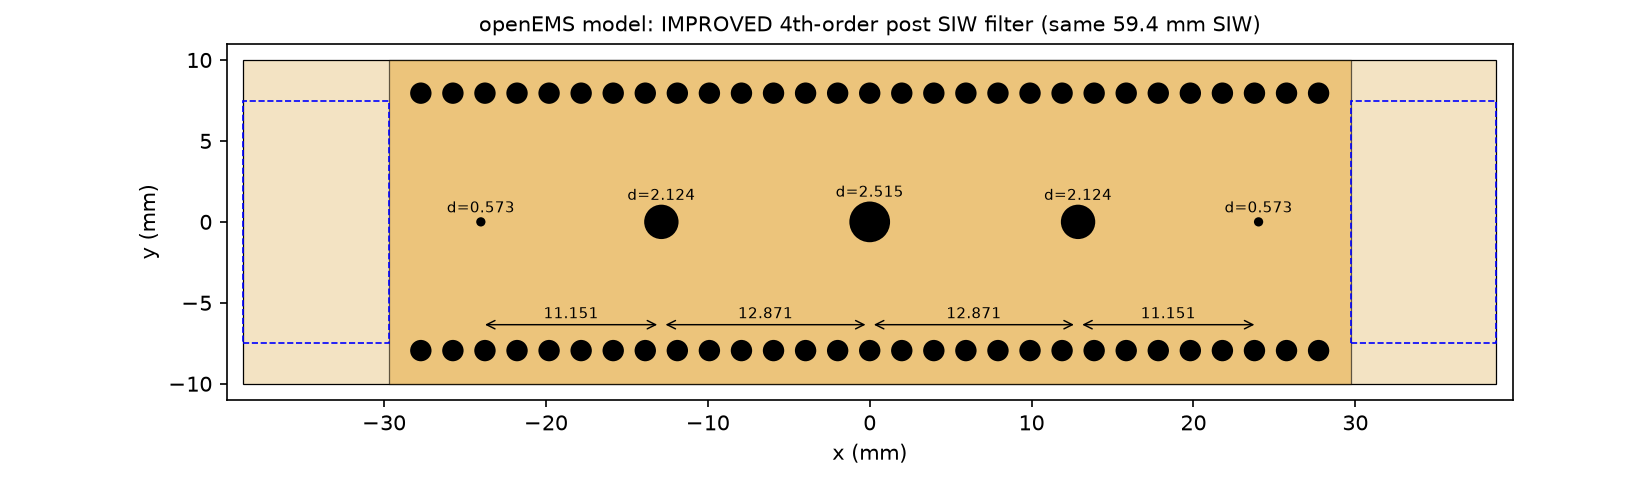
\includegraphics[width=0.49\textwidth]{geom_improved.png}\hfill
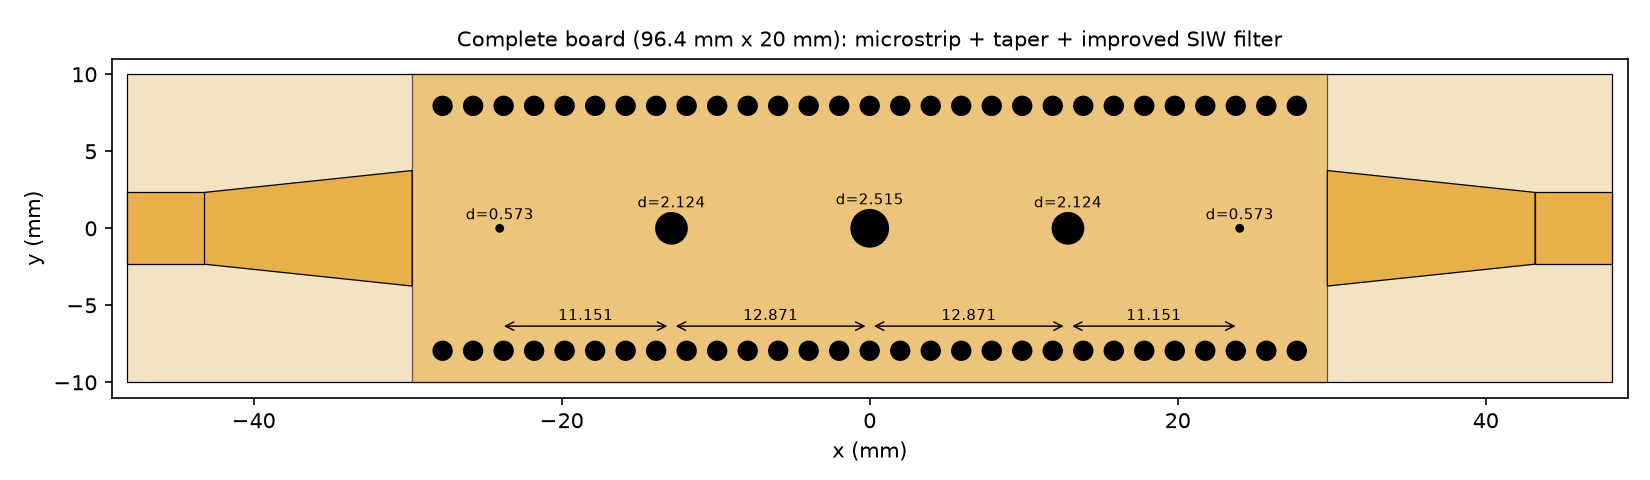
\includegraphics[width=0.49\textwidth]{geom_board.png}
\caption{openEMS models (top view). Left: proposed 4th-order post filter in the \SI{59.4}{mm} SIW of~\cite{bandar2022} (dashed: waveguide-port feeds). Right: complete \SI{96.4}{mm}\,$\times$\,\SI{20}{mm} board with \SI{50}{\Omega} microstrip feeds and linear tapers.}
\label{fig:geom}
\end{figure*}

\section{Validation of the Published Designs}
All seven filters of~\cite{bandar2022} were simulated with their published dimensions and no tuning. Fig.~\ref{fig:val} compares the two 3rd-order Chebyshev filters with the values tabulated in~\cite{bandar2022}, and Table~\ref{tab:val} summarises all designs. Of the 38 tabulated values, 18 (47\,\%) agree at exactly the same frequency and 33 (87\,\%) agree within $\pm$\SI{50}{MHz} ($\pm$0.5\,\%). The band-edge values lie on steep skirts, where a 0.5\,\% shift between two solvers changes $|S_{21}|$ by several decibels; the mesh study shows that this offset is not a discretisation error of the present model.

\begin{figure}[!t]
\centering
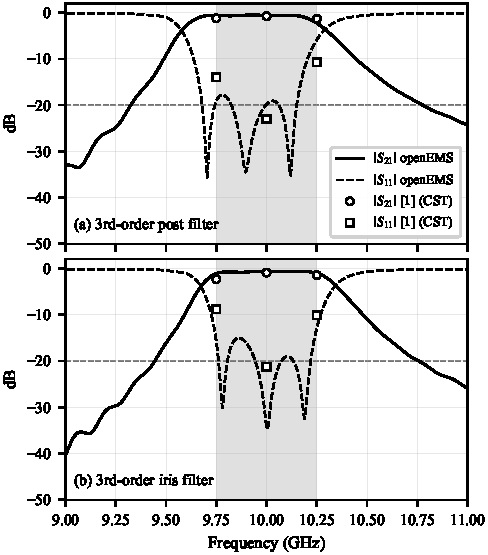
\includegraphics[width=\columnwidth]{fig_validation.pdf}
\caption{Published 3rd-order Chebyshev filters simulated with openEMS (lines) and the values reported in~\cite{bandar2022} (markers). Shaded: specified pass band; dashed: $-20$~dB.}
\label{fig:val}
\end{figure}

\begin{table}[!t]
\caption{openEMS Results of the Published Filters}
\label{tab:val}
\centering
\setlength{\tabcolsep}{2.6pt}
\begin{tabular}{@{}lcccccc@{}}
\toprule
Filter$^\ast$ & $f_0$ & BW$_\mathrm{3dB}$ & \multicolumn{2}{c}{IL at 10 GHz (dB)} & \multicolumn{2}{c}{RL at 10 GHz (dB)}\\
 & (GHz) & (MHz) & openEMS & \cite{bandar2022} & openEMS & \cite{bandar2022}\\
\midrule
Post-3B & 9.92 & 490 & 0.65 & 0.68 & 30.2 & 45.0\\
Post-3C & 9.94 & 700 & 0.62 & 0.78 & 19.8 & 23.0\\
Iris-3B & 9.99 & 470 & 0.77 & 0.52 & 28.3 & 20.0\\
Iris-3C & 10.01 & 660 & 0.59 & 0.89 & 34.5 & 21.2\\
Post-5C & 9.94 & 550 & 1.13 & 0.20 & 19.6 & 32.0\\
Iris-5C & 9.98 & 520 & 1.18 & 0.21 & 22.1 & 28.0\\
Iris-3C, vias & 9.98 & 700 & 0.58 & 0.81 & 17.9 & 30.0\\
\bottomrule
\multicolumn{7}{@{}l}{\footnotesize $^\ast$B: Butterworth; C: Chebyshev 0.1~dB.}
\end{tabular}
\end{table}

All centre frequencies lie within 0.8\,\% of 10~GHz, the responses show the designed orders, the post filter is wider than the iris filter, and replacing the iris walls by small vias leaves the response nearly unchanged, as stated in~\cite{bandar2022}. One discrepancy stands out: the 5th-order filters are reported with 0.2~dB insertion loss, less than the 3rd-order filters of the same work. This is not physically possible with $\tan\delta=0.0012$; Cohn's estimate (1.05~dB) and openEMS (1.13 and 1.18~dB) agree, which suggests that the published 5th-order results were obtained with reduced losses.

\section{Improved Design}
\subsection{Diagnosis}
In openEMS the published 3rd-order Chebyshev post filter reaches $\mathrm{RL}\ge20$~dB only between 9.68 and 10.14~GHz; inside the specified band the return loss falls to 5.8~dB and the insertion loss rises to 2.26~dB. Two causes add up: the 0.1~dB ripple limits the return loss to 16.4~dB even for an ideal filter, and the post diameters in~\cite{bandar2022} were read from Marcuvitz's chart~\cite{marcuvitz1951}.

\subsection{Full-wave inverter extraction}
A single centred post was simulated (lossless) for ten diameters from 0.4 to \SI{3.0}{mm}. After de-embedding to the post plane, its T-equivalent and inverter parameters are~\cite{matthaei1980,uher1993}
\begin{gather}
jX_s=\frac{1-S_{21}+S_{11}}{1-S_{11}+S_{21}},\qquad jX_p=\frac{2S_{21}}{(1-S_{11})^2-S_{21}^2},\\
\varphi=-\arctan(2X_p+X_s)-\arctan X_s,\\
\frac{K}{Z_0}=\left|\tan\!\left(\tfrac{\varphi}{2}+\arctan X_s\right)\right|.
\end{gather}
Fig.~\ref{fig:K} shows the result. The posts of~\cite{bandar2022} give $K/Z_0=0.379$ and 0.134 instead of the required 0.366 and 0.127, i.e.\ couplings that are 4--6\,\% too strong.

\begin{figure}[!t]
\centering
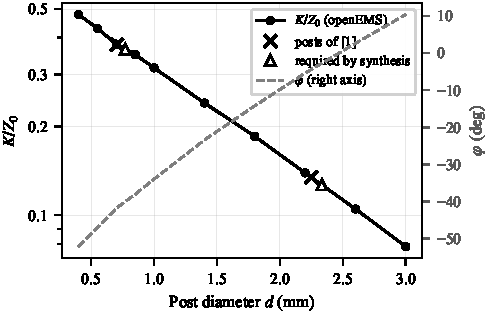
\includegraphics[width=\columnwidth]{fig_K.pdf}
\caption{Full-wave inverter value $K/Z_0$ and phase $\varphi$ of a centred post at 10~GHz versus its diameter, with the posts of~\cite{bandar2022} and the values required by the synthesis.}
\label{fig:K}
\end{figure}

\subsection{Re-synthesis}
The ripple was lowered to 0.03~dB ($\mathrm{RL}_\mathrm{min}=21.6$~dB) over a slightly widened ripple band of 9.72--10.28~GHz. The post diameters were interpolated from $K(d)$, the spacings computed from (3) with the extracted phases, and a short loop rescaled the spacings by $\lambda_g(10\,\mathrm{GHz})/\lambda_g(f_c)$ until the response was centred. Three variants were produced (Table~\ref{tab:imp}). The final 4th-order filter has five posts of 0.5731, 2.1243 and \SI{2.5149}{mm} diameter (symmetric) with spacings of 11.1515 and \SI{12.8709}{mm}; it converged in two full-wave runs and fits in the original \SI{59.4}{mm} SIW.

\begin{table}[!t]
\caption{Published and Improved Post Filters (openEMS)}
\label{tab:imp}
\centering
\setlength{\tabcolsep}{2.6pt}
\begin{tabular}{@{}lcccccc@{}}
\toprule
Design & Order/ & RL$_\mathrm{min}$ & IL$_\mathrm{max}$ & BW$_\mathrm{3dB}$ & \multicolumn{2}{c}{Rejection (dB)}\\
 & ripple & (dB) & (dB) & (MHz) & 9 GHz & 11 GHz\\
\midrule
\cite{bandar2022}, own table & 3/0.1 & 10.7 & 1.33 & -- & -- & --\\
\cite{bandar2022} in openEMS & 3/0.1 & 5.8 & 2.26 & 700 & 33.1 & 24.3\\
Variant A & 3/0.02 & 22.7 & 0.48 & 1030 & 25.3 & 12.2\\
Variant B & 3/0.03 & 22.2 & 0.52 & 910 & 27.2 & 15.4\\
\textbf{Proposed (C)} & \textbf{4/0.03} & \textbf{21.7} & \textbf{0.82} & \textbf{715} & \textbf{46.2} & \textbf{29.8}\\
\bottomrule
\multicolumn{7}{@{}l}{\footnotesize RL$_\mathrm{min}$, IL$_\mathrm{max}$: worst values within 9.75--10.25~GHz.}
\end{tabular}
\end{table}

\subsection{Results}
Fig.~\ref{fig:imp} compares the published and the proposed filter under identical conditions. The proposed design keeps $|S_{11}|$ below $-21.7$~dB across the whole specified band, with four visible reflection zeros, and its worst in-band insertion loss is 0.82~dB instead of 2.26~dB. Variants A and B show that the corrected post sizes and the lower ripple alone already restore the match, but with three resonators the skirts become gentle (12--15~dB rejection at 11~GHz). The fourth resonator restores the selectivity (46/30~dB at 9/11~GHz) at the cost of about 0.25~dB more mid-band loss (0.68~dB); a 5th order would add further loss (about 1.1~dB) without a need for more selectivity.

\begin{figure}[!t]
\centering
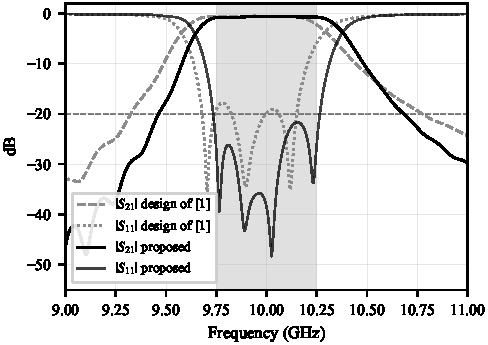
\includegraphics[width=\columnwidth]{fig_improved.pdf}
\caption{Published 3rd-order post filter~\cite{bandar2022} and proposed 4th-order filter, both simulated in openEMS with waveguide ports.}
\label{fig:imp}
\end{figure}

\section{Transition and Complete Board}
The \SI{50}{\Omega} strip on the substrate is \SI{4.66}{mm} wide~\cite{hammerstad1975}. The board length of~\cite{bandar2022} leaves \SI{18.49}{mm} per side, used for a \SI{5}{mm} feed and a \SI{13.49}{mm} linear taper~\cite{deslandes2010}. A back-to-back sweep of the taper width (5.5--\SI{8.5}{mm}) gave an optimum of \SI{7.5}{mm}, with $|S_{11}|<-21.4$~dB from 9 to 11~GHz and 0.12~dB loss. The complete boards were then simulated with microstrip ports (Fig.~\ref{fig:board}, Table~\ref{tab:board}). With identical tapers, the proposed filter improves the worst in-band return loss from 4.0 to 17.7~dB and the worst insertion loss from 2.48 to 0.74~dB. The return loss of the proposed board dips below 20~dB near 10.25~GHz because the two taper reflections add to that of the filter; co-tuning the outer posts with the taper is left for future work.

\begin{figure}[!t]
\centering
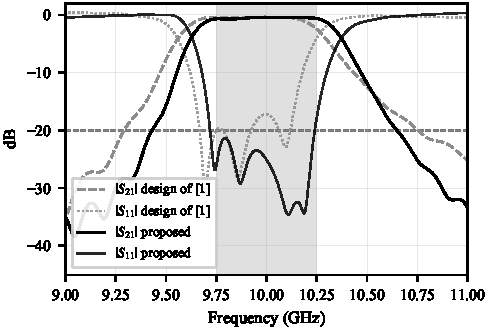
\includegraphics[width=\columnwidth]{fig_board.pdf}
\caption{Complete \SI{96.4}{mm}\,$\times$\,\SI{20}{mm} boards with \SI{50}{\Omega} microstrip ports.}
\label{fig:board}
\end{figure}

\begin{table}[!t]
\caption{Complete Boards with Microstrip Ports (openEMS)}
\label{tab:board}
\centering
\setlength{\tabcolsep}{3pt}
\begin{tabular}{@{}lcccccc@{}}
\toprule
Board & RL$_\mathrm{min}$ & IL$_\mathrm{max}$ & IL$_{10\,\mathrm{GHz}}$ & BW$_\mathrm{3dB}$ & \multicolumn{2}{c}{Rej. (dB)}\\
 & (dB) & (dB) & (dB) & (MHz) & 9 GHz & 11 GHz\\
\midrule
Filter of~\cite{bandar2022} & 4.0 & 2.48 & 0.37 & 695 & 35.4 & 25.1\\
Proposed filter & 17.7 & 0.74 & 0.51 & 725 & 35.0 & 33.4\\
\bottomrule
\end{tabular}
\end{table}

\section{Conclusion}
A published study of post and iris SIW band-pass filters at X-band was reproduced with the open-source FDTD solver openEMS: 87\,\% of the tabulated values agree within $\pm$0.5\,\% in frequency and all qualitative conclusions are confirmed, while the reported 0.2~dB loss of the 5th-order filters was shown to be unattainable. The weak band-edge match of the published post filter was traced to a 0.1~dB ripple and to chart-read post sizes. Replacing the chart by a full-wave extraction of the post inverter and phase gave a 4th-order filter in the same SIW with a return loss above 21.7~dB, an insertion loss below 0.82~dB over the full 500~MHz band and clearly better rejection. The results are simulations; fabrication with TRL-calibrated measurement and a tolerance analysis are the next steps. All models are Python scripts that run with free software, so every result can be reproduced.

\section*{Acknowledgment}
The authors thank Dr. Nagavel B, Department of Electronics and Communication Engineering, NITK Surathkal, for guiding this work, and the developers of openEMS for making a full-wave solver freely available.

\begin{thebibliography}{00}
\bibitem{bandar2022} H. Bandar and N. T\"urker Tokan, ``Comparison of post and iris substrate integrated waveguide band-pass filters for X-band applications,'' \textit{Sigma J. Eng. Nat. Sci.}, vol.~40, no.~1, pp.~45--56, 2022.
\bibitem{deslandes2001} D. Deslandes and K. Wu, ``Integrated microstrip and rectangular waveguide in planar form,'' \textit{IEEE Microw. Wireless Compon. Lett.}, vol.~11, no.~2, pp.~68--70, Feb. 2001.
\bibitem{deslandes2003} D. Deslandes and K. Wu, ``Single-substrate integration technique of planar circuits and waveguide filters,'' \textit{IEEE Trans. Microw. Theory Techn.}, vol.~51, no.~2, pp.~593--596, Feb. 2003.
\bibitem{bozzi2011} M. Bozzi, A. Georgiadis, and K. Wu, ``Review of substrate-integrated waveguide circuits and antennas,'' \textit{IET Microw. Antennas Propag.}, vol.~5, no.~8, pp.~909--920, 2011.
\bibitem{chen2014} X.-P. Chen and K. Wu, ``Substrate integrated waveguide filters: Design techniques and structure innovations,'' \textit{IEEE Microw. Mag.}, vol.~15, no.~6, pp.~121--133, Sep. 2014.
\bibitem{matthaei1980} G. L. Matthaei, L. Young, and E. M. T. Jones, \textit{Microwave Filters, Impedance-Matching Networks, and Coupling Structures}. Dedham, MA, USA: Artech House, 1980.
\bibitem{liebig2013} T. Liebig, A. Rennings, S. Held, and D. Erni, ``openEMS -- a free and open source equivalent-circuit (EC) FDTD simulation platform supporting cylindrical coordinates suitable for the analysis of traveling wave MRI applications,'' \textit{Int. J. Numer. Model.}, vol.~26, no.~6, pp.~680--696, 2013.
\bibitem{cassivi2002} Y. Cassivi, L. Perregrini, P. Arcioni, M. Bressan, K. Wu, and G. Conciauro, ``Dispersion characteristics of substrate integrated rectangular waveguide,'' \textit{IEEE Microw. Wireless Compon. Lett.}, vol.~12, no.~9, pp.~333--335, Sep. 2002.
\bibitem{xu2005} F. Xu and K. Wu, ``Guided-wave and leakage characteristics of substrate integrated waveguide,'' \textit{IEEE Trans. Microw. Theory Techn.}, vol.~53, no.~1, pp.~66--73, Jan. 2005.
\bibitem{cohn1959} S. B. Cohn, ``Dissipation loss in multiple-coupled-resonator filters,'' \textit{Proc. IRE}, vol.~47, no.~8, pp.~1342--1348, Aug. 1959.
\bibitem{pozar2011} D. M. Pozar, \textit{Microwave Engineering}, 4th ed. Hoboken, NJ, USA: Wiley, 2011.
\bibitem{marcuvitz1951} N. Marcuvitz, \textit{Waveguide Handbook}. New York, NY, USA: McGraw-Hill, 1951.
\bibitem{uher1993} J. Uher, J. Bornemann, and U. Rosenberg, \textit{Waveguide Components for Antenna Feed Systems: Theory and CAD}. Norwood, MA, USA: Artech House, 1993.
\bibitem{hammerstad1975} E. O. Hammerstad, ``Equations for microstrip circuit design,'' in \textit{Proc. 5th Eur. Microw. Conf.}, 1975, pp.~268--272.
\bibitem{deslandes2010} D. Deslandes, ``Design equations for tapered microstrip-to-substrate integrated waveguide transitions,'' in \textit{IEEE MTT-S Int. Microw. Symp. Dig.}, 2010, pp.~704--707.
\end{thebibliography}

\end{document}
